\documentclass[tikz,border=10pt]{standalone}

\begin{document}
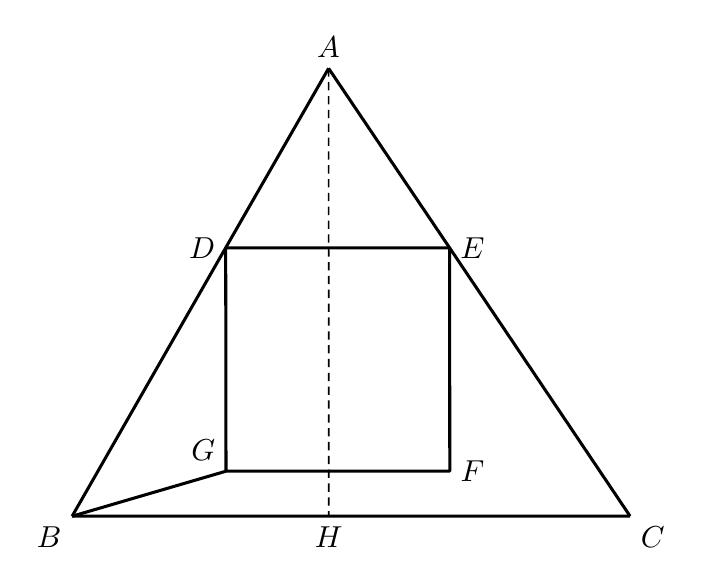
\begin{tikzpicture}[line join=round, line width=1.1pt,
  every node/.style={font=\fontsize{11}{13.2}\selectfont}]
\coordinate (A) at (-0.291,2.854);
\coordinate (B) at (-3.548,-2.834);
\coordinate (C) at (3.537,-2.832);
\coordinate (D) at (-1.598,0.575);
\coordinate (E) at (1.246,0.574);
\coordinate (F) at (1.248,-2.261);
\coordinate (G) at (-1.594,-2.262);
\coordinate (H) at (-0.289,-2.833);

  

  
  \draw (A) -- (D) -- (B);
  \draw (A) -- (E) -- (C);
  \draw (B) -- (H) -- (C);

  
  \draw (D) -- (E) -- (F) -- (G) -- cycle;

  
  \draw (B) -- (G);

  
  \draw[line width=0.6pt, dash pattern=on 3pt off 2pt] (A) -- (H);

  
  \node[above] at (A) {$A$};
  \node[below left] at (B) {$B$};
  \node[below right] at (C) {$C$};
  \node[below] at (H) {$H$};
  \node[left] at (D) {$D$};
  \node[right] at (E) {$E$};
  \node[right] at (F) {$F$};
  \node[above left] at (G) {$G$};
\end{tikzpicture}
\end{document}